\section{Theorie}

\subsection{CBCast Algorithmus}

In einem Netzwerk laufen verschiedene Prozesse auf verschiedenen Knoten und teilen sich keinen Speicherplatz. Die Interaktion zwischen den verschiedenen Prozessen läuft soweit ausschließlich über die Weitergabe von Nachrichten und kein Prozess kennt das Verhalten anderer Prozesse \cite{CBCAST_1}. Der CBCast (Chain-Based Broadcast) Algorithmus ist ein Algorithmus der im Bereich der verteilten Systeme zum Einsatz kommt und eine Lösung für genau diese Prozessinteraktion implementiert. Genutzt wie zum Beispiel vom ISIS Projekt \cite{isis_project} hat er sich in der Vergangenheit bereits mehrfach renommiert. 

\begin{figure}[htbp]
\begin{center}
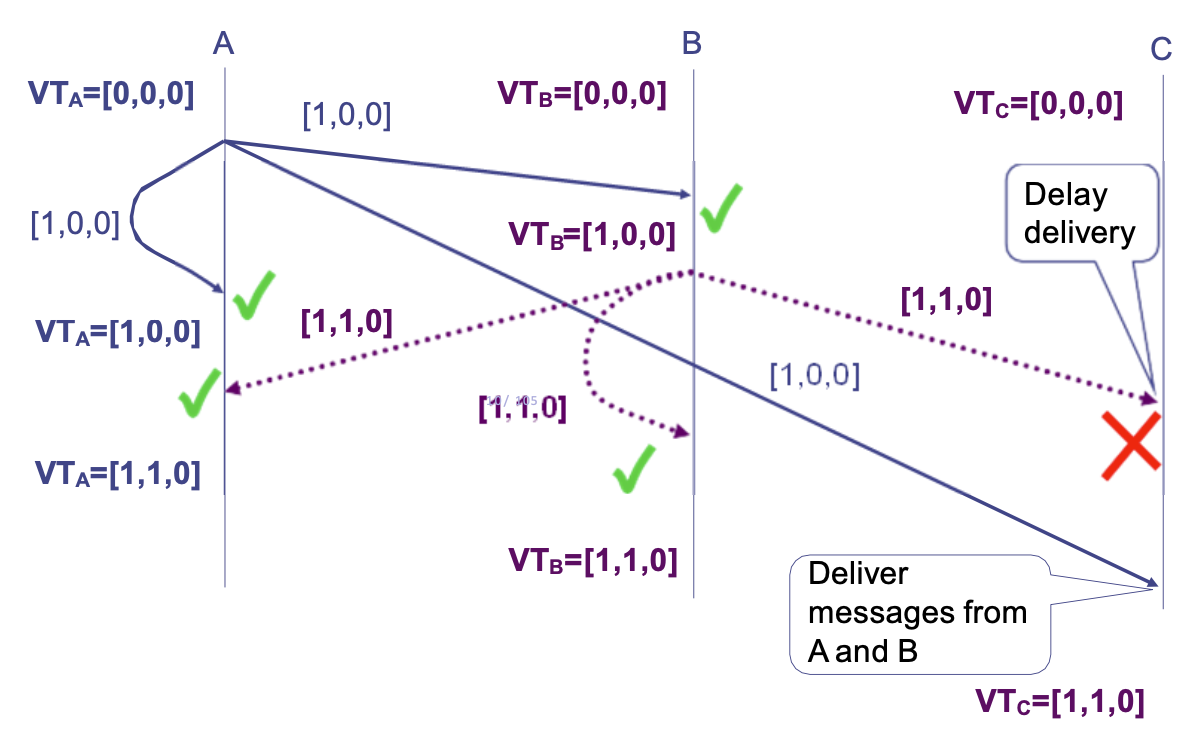
\includegraphics[scale=0.4]{Latex/Bilder/cbcast_2.png}
\caption{\label{fig:cbcastFunction} CBCAST \cite{Aufgabenstellung}} 
\end{center}
\end{figure}

In Abb. \ref{fig:cbcastFunction} zu sehen ist ein beispielhafter Ablauf des CBCASTs mit drei Prozessen 'A', 'B' und 'C'. 

\subsection{Kommunikationseinheit}

\subsection{Vektoruhr-ADT}

\subsection{Vektoruhr Zentrale/Tower}

\subsection{Ungeordneter Multicast}
